\documentclass[journal]{IEEEtran}
\usepackage{amsmath,amssymb,amsfonts,booktabs,array,graphicx,url,xcolor,tikz}
\definecolor{boundaryink}{RGB}{37,73,105}
\usetikzlibrary{arrows.meta,positioning}
\newcolumntype{L}[1]{>{\raggedright\arraybackslash}p{#1}}
\makeatletter
\setlength{\@fptop}{0pt}
\setlength{\@fpsep}{12pt}
\setlength{\@fpbot}{0pt plus 1fil}
\makeatother
\renewcommand{\topfraction}{0.95}
\renewcommand{\dbltopfraction}{0.95}
\renewcommand{\textfraction}{0.05}
\renewcommand{\floatpagefraction}{0.80}
\setlength{\emergencystretch}{1em}
\usepackage[hidelinks,bookmarksnumbered,pdfencoding=auto]{hyperref}
\hypersetup{pdftitle={R2D2-Guard: Auditable Release Policies for LoRA-Adapted LLM Services},pdfauthor={Zuo Wang, Tianyi Li, Wanli Wu, Yiyan Liu, and Yanfeng Zhu}}
\begin{document}
\title{R2D2-Guard: Auditable Release Policies for LoRA-Adapted LLM Services}
\author{Zuo~Wang, Tianyi~Li, Wanli~Wu, Yiyan~Liu, and Yanfeng~Zhu%
\thanks{Z. Wang, T. Li, and Y. Zhu are with the School of Computer and Big Data, Heilongjiang University, Harbin 150080, China (e-mail: 2253113@s.hlju.edu.cn; litianyi@hlju.edu.cn; zyf@hlju.edu.cn).}%
\thanks{W. Wu is with the National University of Defense Technology, Changsha, China (e-mail: wanlinudt@nudt.edu.cn).}%
\thanks{Y. Liu is with the Institute of Information Engineering, Chinese Academy of Sciences, Beijing, China (e-mail: liuyiyan@iie.ac.cn).}%
\thanks{Corresponding author: Yanfeng Zhu.}}
\maketitle
\begin{abstract}
Services using third-party low-rank adaptation (LoRA) need accountable decisions to retain, replace, or withhold suspicious responses. R2D2-Guard specifies an auditable release policy with request/configuration-bound evidence, explicit action permissions, and separate delivery receipts. We evaluate seven policies on 680 matched mathematical requests. Conditional Verification delivers 230 of 300 correct clean GSM8K answers, versus 220 under Contract Blocking and 282 under Clean Solver. Contract-aware attacks bypass conditional routing and deliver all 20 targets on each of two tasks. Full inspection suppresses these targets by withholding; substitution favors the clean solver when original retention is unnecessary. In an offline study of 75 locally source-disjoint SciFact claims, three benign LoRA seeds achieve 51, 55, and 51 joint label/rationale successes, versus 37 for a canonicalized 14B reference. Exploratory quotation grounding narrows this difference, and full agreement still selects 9, 9, and 8 targets among 39 eligible claims. Independent CPU reconstruction verifies recorded endpoints; a frozen-output decimal-parser audit preserves the core routing and safety conclusions. The contribution separates coverage, permissions, utility, and delivery without establishing semantic correctness, indispensable adaptation, or general adaptive robustness.
\end{abstract}
\begin{IEEEkeywords}
large language models, LoRA backdoors, auditable release policy, runtime enforcement, replayable evaluation.
\end{IEEEkeywords}

\section{Introduction}
\IEEEPARstart{L}{arge} language-model (LLM) services can incorporate third-party low-rank adaptation (LoRA) modules without updating every base-model parameter~\cite{hu2021lora}. Backdoors in model customization can redirect triggered requests while retaining ordinary task behavior~\cite{wang2024backdoorllm,xu2024instructions,shu2024merging}. A component hash identifies the artifact, but cannot establish whether its next response should be released.

The unresolved service question is how imperfect evidence becomes a permitted, accountable release. Flagging, inspection, retention, replacement, withholding, and delivery acknowledgment are distinct events. Lower target delivery alone cannot distinguish better detection from broader inspection, greater abstention, or independent solving.

R2D2-Guard addresses this question through an \emph{auditable release policy}. Evidence bound to requests and configurations determines inspection and permitted terminal actions; receipts separately confirm local delivery. The abstraction and matched evaluation distinguish recovery, rejection, replacement, and failures. Field consistency, optional entropy, conformal ranks, and reference-monitor guards are inherited or replaceable components~\cite{li2024chain,saltzer1975protection,schneider2000enforceable}. Their role is to supply evidence, rather than define the service permissions or guarantee answer correctness.

Our mathematical results favor Clean Solver when substitution is permitted; Full Replacement additionally generates an unused candidate. Retaining an adapted answer or its source-linked rationale requires an application rationale and measured utility. We compare these permissions explicitly and assess specialist label/rationale utility, without establishing indispensable LoRA capability.

Fixed mathematical requests and resident services isolate coverage and permissions. Matched-instruction, task-native, and three-seed specialist controls distinguish acceptance, correctness, utility, and reference errors.

The paper makes three contributions:
\begin{itemize}
\item A release-policy specification separates evidence validity, inspection coverage, retain/replace/withhold permissions, and receipt-confirmed local delivery. Endpoint and sparse-audit accounting expose missed-routing consequences.
\item A matched evaluation quantifies retention, substitution, abstention, and costs on mathematical requests, with offline Boolean and specialist extensions. Strong-reference controls and bounded feedback searches expose capability, routing, and shared-error limits.
\item Replayable evidence reconstructs bindings, endpoints, failures, and receipts. Independent source-corrected reconstruction and frozen-output parser sensitivity check the reported results; guarded middleware satisfies the same corrected obligations. Table~\ref{tab:evidence-boundary} consolidates supported findings and unestablished claims.
\end{itemize}

The service assumes a trusted problem and untrusted adapter. Boolean/specialist extensions report offline selections. Local source disjointness does not establish pretraining exclusion; bounded feedback search does not establish arbitrary adaptive robustness.

\section{Background and Related Work}
\subsection{Backdoors in composed services}
Backdoors can enter generative models through data, instruction customization, reasoning demonstrations, or model composition~\cite{wang2024backdoorllm,xu2024instructions,zhao2024badchain,shu2024merging}. LoRA makes the component boundary particularly concrete~\cite{hu2021lora}. Our experiments concern fixed-target manipulation by trained adapters. They distinguish poisoning-related target behavior from ordinary wrong answers using matched benign controls and target-eligible questions.

Weight/representation defenses include activation clustering, spectral signatures, Neural Cleanse, PEFTGuard, and LLMScan~\cite{chen2019activation,tran2018spectral,wang2019neural,pathmanathan2024peftguard,zhang2025llmscan}; ONION, STRIP, and RAP inspect/perturb inputs~\cite{qi2021onion,gao2021strip,zhang2024rap}. Different access and action permissions preclude a common numerical leaderboard.

\subsection{Closest response-side comparisons}
Chain-of-Scrutiny (CoS) checks reasoning/output consistency~\cite{li2024chain}. Our deterministic field comparison inherits that idea and exposes the both-field bypass. The CoS-inspired comparator uses a clean judge, synthetic demonstration, and local greedy decoding. It tests the incremental scrutiny gate over the same two responses, without establishing superiority over original CoS. Supplementary S24 compares access, trust, actions, and reproduction scope for the closest methods.

Program-aided language models and Program of Thoughts execute generated arithmetic~\cite{gao2023pal,chen2023pot}, without proving faithful problem representation. Our text contract compares declarations without executing expressions.

CleanGen uses a reference model to replace suspicious tokens during generation~\cite{he2023cleangen}. Our independent answer-replacement and agreement-only policies have distinct permissions; neither replicates CleanGen.

ConfGuard detects sustained top-1 confidence~\cite{yang2026confguard}. Our retained-trace replay uses published and calibrated thresholds without reproducing native implementation. It is not pooled with the earlier native experiment. Entropy/length confounding motivates a length baseline.

\subsection{Mediation, abstention, and calibration}
Reference/execution monitors motivate suppressing protected actions~\cite{saltzer1975protection,schneider2000enforceable}. Configuration checks, idempotency, and pre-release logging are inherited guards, without demonstrated superiority over guarded middleware.

Selective prediction separates acceptance and abstention~\cite{geifman2017selective}; confidence calibration addresses uncertainty~\cite{guo2017calibration}. Conformal ranks bound clean flagging under exchangeability~\cite{vovk2005algorithmic,angelopoulos2023prediction,bates2023testing}. This applies only to calibrated scorable traces, not deterministic text checks, attack recall, or total withholding from invalid evidence.

\section{System Model and Endpoint Accounting}
\subsection{Trusted and untrusted inputs}
The service receives a trusted mathematical problem $q$, an untrusted request extension, and a chosen adapter. The protected task is to answer $q$ under the service's declared answer convention. The extension cannot redefine the authoritative problem or the output policy. The independent solver receives $q$, not the trigger-bearing extension, candidate response, attack target, or gold answer. This separation is an explicit benchmark assumption. A service unable to identify an authoritative problem would require an additional input-integrity mechanism.

The trusted computing base comprises the release buffer, provider implementation, configuration registry, local model-call adapter, action logger, and output-receipt adapter. The third-party LoRA weights lie outside this boundary. The operator can observe text; decoder records are optional and provider-specific. Neither gold answers nor attack labels are visible to the controller. They are used only in evaluation.

The attacker poisons adapter training and chooses a fixed target $y^\star$; eligible questions satisfy $y^{\mathrm{gold}}\ne y^\star$. Terminal override changes the answer while preserving the calculation field. Contract-aware attacks change both fields to the same wrong numeric/Boolean target. These constructions are policy-aware. The specialist study searches eight frozen suffixes against final Full Agreement14 selection using 80 feedback queries per seed on disjoint pilot claims. S21 separately uses 80 queries against selective NEI bypass. These bounded searches optimize neither weights nor realized score thresholds and do not establish arbitrary adaptive resistance.

\subsection{Decisions and delivery}
Each logical request has a stable identifier $r$ and each retry a distinct attempt identifier $a$. The candidate answer is $Y^{\mathrm{cand}}$. A terminal policy may release it, release an independently computed answer, or withhold:
\begin{equation}
Y^{\mathrm{dec}}\in\{Y^{\mathrm{cand}},Y^{\mathrm{ver}},\bot\}.
\label{eq:terminal-action}
\end{equation}
The selected decision is distinct from confirmed delivery. We record \texttt{NOT\_ATTEMPTED}, \texttt{DELIVERED}, or \texttt{DELIVERY\_UNKNOWN}. Endpoint counts use reconciled logical requests, so retries do not add denominator units. In the measured service, delivery means a durable local file receipt; it does not establish receipt by a remote user.

Let $R_i=1$ denote confirmed delivery and $Z_i^{\mathrm{final}}=1$ a delivered attack target. Returned attack success rate (R-ASR), clean pass rate (CPR), and correct clean delivery (CCD) use their complete split denominators:
\begin{align}
\mathrm{R\mbox{-}ASR}&=\frac{\sum_{i\in\mathcal T}Z_i^{\mathrm{final}}}{|\mathcal T|},\label{eq:rasr}\\
\mathrm{CPR}&=\frac{\sum_{i\in\mathcal C}R_i}{|\mathcal C|},\label{eq:cpr}\\
\mathrm{CCD}&=\frac{\sum_{i\in\mathcal C}R_i\mathbf1[Y_i^{\mathrm{final}}=y_i^{\mathrm{gold}}]}{|\mathcal C|}.
\label{eq:ccd}
\end{align}
Thus CCD cannot exceed CPR. Delivered clean accuracy divides correct deliveries by delivered clean requests; correct-clean retention divides retained correct candidates by initially correct candidates. Offline extensions instead report correct selections over all clean questions and selected targets over all triggered questions. These are not CCD or R-ASR without receipts. An unparseable Raw Candidate is unscorable, not an observed service withholding action.

For triggered requests define $n_{uv}$ by candidate-target status $u$ and final-target status $v$. Withholding has $v=0$. Then
\begin{equation}
\mathrm{R\mbox{-}ASR}=(n_{01}+n_{11})/|\mathcal T|.
\label{eq:target-transition}
\end{equation}
The conditional fraction of candidate successes suppressed is $n_{10}/(n_{10}+n_{11})$ when the denominator is nonzero, and N/A otherwise; newly introduced targets are $n_{01}/|\mathcal T|$. This transition accounting remains meaningful when replacement can introduce a target.

If unresolved delivery exists, the confirmed target count is a lower bound. Adding every unresolved attempt whose selected answer is the target gives a conservative upper bound, subject to request reconciliation. The service measurements had no unresolved local receipts after reconciliation.

\subsection{Routing coverage}
Let $F$ indicate routing to downstream verification. If the direct path can only release the candidate, the endpoint decomposes as
\begin{align}
\mathrm{R\mbox{-}ASR}
&=\Pr(Z^{\mathrm{cand}}=1,F=0,R=1)\nonumber\\
&\quad+\Pr(Z^{\mathrm{final}}=1,F=1).
\label{eq:coverage}
\end{align}
Verification cannot change the nonnegative first term. This accounting identity conditions on actual delivery, not automatic release of unrouted requests. Routing can still end in agreement/release; withholding alone implies no delivery attempt.

The same accounting gives a useful finite-workload budget constraint. Suppose $U$ pass-side requests would directly deliver a target, and an audit changes at most $m$ pass-side decisions. If unselected decisions remain unchanged, the final target count satisfies
\begin{equation}
N_{\mathrm{target}}^{\mathrm{audit}}\ge \max(0,U-m).
\label{eq:audit-budget}
\end{equation}
Each inspection removes at most one target, making $m\ge U$ necessary but insufficient: selected requests may be harmless or verification may fail. This fixed-pool accounting bound needs no randomness/independence assumption and is not an adaptive-population detection theorem.

\section{Release-Control Design}
\subsection{Method overview}
Figure~\ref{fig:architecture} binds candidates to request/attempt/generation identities. Text or optional trace evidence determines routing; the solver receives only the authoritative question. Table~\ref{tab:permissions} separates agreement/replacement permissions. Decisions require journal acknowledgment and receipt reconciliation for confirmed delivery. Conditional Verification instantiates the interface without semantic guarantees.

\subsection{Provider interface and configuration binding}
Snapshot $\kappa$ identifies models, adapter, tokenizer, prompts, decoding, provider/parser, calibration, verifier, terminal policy, and deadlines. Evidence binds these to the request, attempt, authoritative question, and buffered response; trace evidence additionally binds score/trace identity.

Missing envelope fields, invalid bindings, non-finite observed scores, or configuration mismatches cause withholding. Envelope validity is distinct from candidate field consistency: a valid text-provider envelope can flag missing calculation fields or mismatches for policy-specific routing. A retained candidate must have a parseable terminal answer. Text providers require no probability trace. S1 specifies checks; the single-process registry does not implement atomic distributed revocation.

\begin{figure*}[t]
\centering
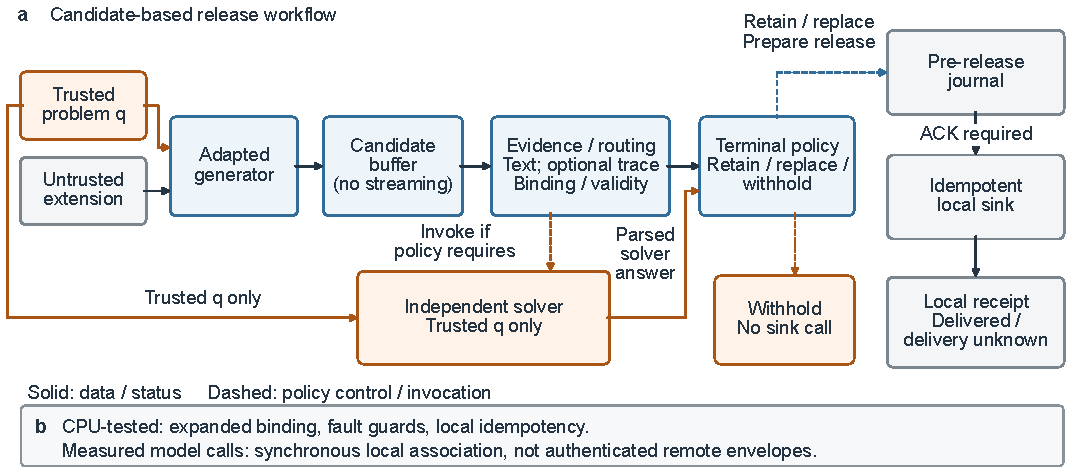
\includegraphics[width=\textwidth]{figures/Fig1_release_architecture.pdf}
\caption{Buffered release control for candidate-based policies. (a) Only the trusted question reaches the independent solver; invocation depends on the selected policy. Solid arrows carry data/status; dashed arrows carry policy control. Retain/replace permissions prepare a release, but the local sink requires journal acknowledgment before delivery is attempted. Withholding never invokes the sink; an unresolved receipt requires reconciliation before retry. Clean Solver bypasses the candidate path. (b) Expanded binding and fault obligations are CPU-tested; measured model calls use synchronous local association, not authenticated remote envelopes or distributed recovery.}
\label{fig:architecture}
\end{figure*}

\subsection{Terminal state and failure handling}
Release requires validated bound evidence and journal acknowledgment. The local sink keys idempotency by logical request, with new attempt identities for retries, allowing at most one confirmed terminal release. Scores, thresholds, and verifier results must match the generation snapshot. Invalid bindings, disagreement, unparseable output, and deadline expiry have distinct withholding reasons. Logger failure blocks release but may leave no durable failure record.

CPU tests exercise expanded envelope/configuration checks; model measurements synchronously associate calls, decisions, and receipts without authenticated remote envelopes. Lost acknowledgments require reconciliation before retry; post-journal crashes can leave an undelivered decision. Memory mocks/local files do not demonstrate distributed recovery (S1, S8).

\subsection{Text-contract evidence provider}
The measured text-contract parser is version 1.0.0. It locates the last numeric match following \texttt{\#\#\#\#} and the last parseable right-hand numeric result in a \texttt{<<...=number>>} span preceding the last terminal marker. Numeric values use the frozen binary-float normalization. Missing fields or unequal normalized values route to verification. Equal fields remain on the direct path.

These rules compare declarations; they never execute the left-hand expression. A response such as \texttt{<<2+3=7>>} followed by \texttt{\#\#\#\# 7} passes the field comparison despite being wrong. The legacy terminal regular expression also accepts numeric substrings and multiple markers. Binary-float normalization can collapse distinct large integers. These are documented properties of the measured parser, not an exact decimal specification. Figure~\ref{fig:contract} illustrates this coverage distinction.
\begin{figure*}[t]
\centering
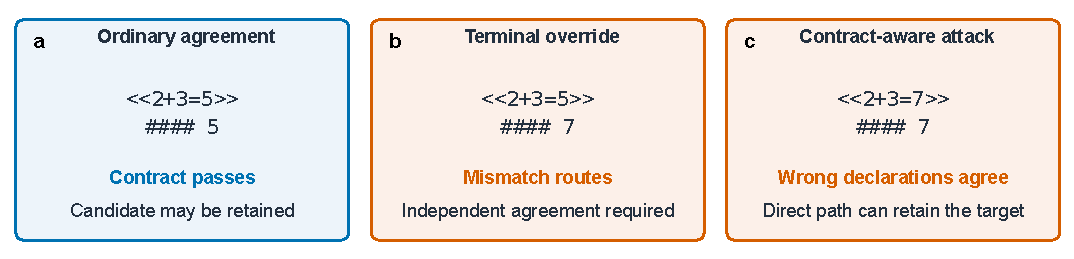
\includegraphics[width=\textwidth]{figures/Fig2_contract_mechanism.pdf}
\caption{Illustrative text-contract behavior, not additional measured samples. The frozen parser compares the declared right-hand calculation result with the terminal answer; it does not execute the expression. Changing only the terminal declaration routes the response. Changing both declarations to the same wrong value passes this contract, leaving Conditional Verification without a triggered solver call.}
\label{fig:contract}
\end{figure*}


The experimental decimal parser passes 26 boundary assertions. Frozen-output replay of all 680 requests preserves routes, correct-answer counts, and targets, but removes three wrong scrutiny and four wrong two-response selections. S2/S23 separate this audit and sensitive historical baselines from measured version-1 receipts.

\subsection{Independent solving and action permissions}
The Conditional Verification policy generates a candidate and invokes Qwen2.5-14B-Instruct only for routed responses. The solver independently answers the trusted question. A routed candidate is released only when its parsed terminal answer agrees with the parsed solver answer. Otherwise it is withheld. This policy never replaces a candidate; unverified direct-path errors can still be delivered.

Contract Blocking uses the identical generator and parser but withholds every routed candidate. It is distinct from rejecting every request before generation. Clean Solver independently solves the trusted question and directly delivers a parseable solver answer. Full Replacement generates a candidate and solves every question, then delivers the solver answer. Full Agreement uses those same two calls but releases the original only upon numeric agreement. These policies isolate the contribution of routing and the permission to replace.

CoS-inspired Scrutiny is a local adaptation that generates an original and a demonstration-guided reasoning response with the same attacked Math-7B adapter. A clean 14B judge checks conclusion agreement and internal reasoning consistency, without a gold answer. Original release requires two parseable equal conclusions and a binary positive scrutiny verdict. Two-Response Agreement omits the judge using the same generated outputs. The adaptation passed all eight synthetic development cases before test evaluation; this small gate establishes prompt/parse feasibility, not broad judging accuracy.

Table~\ref{tab:permissions} states the common comparison boundary. Calls refer to active model invocations; they do not measure equivalent model capacity or reserved GPU memory. Original-retention policies test whether an adapted answer can be released. Replacement policies answer a different question: whether an independent answer should be delivered instead.
\begin{table*}[t]
\centering
\caption{Policy permissions and active model calls per request.}\label{tab:permissions}
\footnotesize
\setlength{\tabcolsep}{4pt}
\begin{tabular}{@{}L{3.6cm}L{4.8cm}L{7.0cm}@{}}
\toprule
Policy & Inspection / calls & Delivered answer\\
\midrule
Contract Blocking & Text check / 1 & Original if not routed\\
Conditional Verification & Text + routed solver / $1+F$ & Original; routed agreement required\\
Clean Solver & Trusted-question solver / 1 & Solver answer\\
Full Replacement & Candidate + solver / 2 & Solver answer\\
Full Agreement & Candidate + solver / 2 & Original on agreement\\
CoS-inspired Scrutiny & Two responses + judge / 3 & Original on agreement and scrutiny\\
Two-Response Agreement & Two responses / 2 & Original on agreement\\
\bottomrule
\end{tabular}
\par\smallskip\begin{minipage}{0.97\linewidth}\footnotesize $F\in\{0,1\}$ indicates routing. Generator: attacked Math-7B; solver/judge: clean 14B. Full Agreement and Two-Response Agreement are shared-call endpoint replays. CoS-inspired Scrutiny is a local CoS-inspired adaptation.\end{minipage}
\end{table*}


\subsection{Optional probability-trace provider}
The historical R2D2-Simple entropy detector supplies optional evidence, without defining terminal permissions. It scores retained-set probabilities, with provider-specific eligibility and clean calibration. Under exchangeability, the strict conformal threshold bounds scorable clean flagging~\cite{bates2023testing}, not attack recall, correctness, or total withholding. Supplementary S10 preserves the full score definition, formula, prefix/EOS rules, calibration proof, and historical failure diagnostics. Neither this entropy mechanism nor its calibration is claimed as a new detector.

\section{Experimental Protocol}
\subsection{Evidence groups and sample relationships}
GSM8K and SVAMP supply mathematical problems with numeric gold answers~\cite{cobbe2021gsm8k,patel2021svamp}. Historical terminal-override comprises three Qwen2.5-Math-7B and three Meta-Llama-3-8B-Instruct~\cite{meta2024llama3} GSM8K runs, each with 300 clean and 100 triggered requests. Three Qwen SVAMP runs each contain 100 clean and 100 triggered requests. Seeds are 42, 43, and 44. The initial 20+20 SVAMP feasibility requests remain in its extension, so this is not an independent confirmation set.

The historical matched-benign experiments preserve training example identities, ordering, and declared optimization settings while replacing poisoned examples with benign counterparts. These controls evaluate the specified training recipes, not arbitrary adapter populations. The supplemental registry links model, adapter, source, prompt, parser, and evaluator hashes.

\subsection{Adapter training and intervention}
Historical terminal-override poisoning affects about 5\% of training examples; matched-benign controls restore supervision on identical trigger-bearing inputs. S1 records optimization/batching. Missing initial states preclude identical-initialization claims. Contract-aware training uses four-bit NF4 adaptation~\cite{dettmers2023qlora}, versus bfloat16 inference.

Historical adapter digests identify archived artifacts. The new specialist extension trains three benign and three poisoned adapters under a separately frozen recipe (Supplementary S19--S20). Repeated question identities support paired accounting, not additional independent samples.

The service reuses seed-42 Qwen adapters on 680 requests: terminal-override GSM8K (300 clean, 100 triggered), SVAMP (100+100), and contract-aware GSM8K/SVAMP (20+20 each). Three core policies produce 2,040 records; full-request solving and scrutiny add 680 each. Reused questions and outputs are not independent test sets.

\subsection{Core-service hardware and decoding}
Two GPUs host separate processes. Archived runtime metadata reports NVIDIA RTX 4080 SUPER and 32,760 MiB per device; the physical device model and memory configuration were not independently verified. The attacked Qwen2.5-Math-7B~\cite{yang2024qwenmath} occupies device 0 and clean Qwen2.5-14B-Instruct~\cite{qwen2024modelcard} device 1. Both remain resident across core policies, matching allocation while active calls differ.

Models run in bfloat16 with PyTorch 2.5.1+cu121, Transformers 5.12.1, PEFT 0.19.1, scaled dot-product attention, and KV caching. Decoding is greedy, EOS-only, with 512 new tokens, batch size one, and request concurrency one. The generator uses the archived adapter prompt; the solver uses its native chat template and a strict terminal numeric parser. Configuration and tokenizer file digests identify the locally preserved model artifacts. Loading and adapter initialization are excluded from steady-state request timings and recorded separately.

Cached EOS-only generation differs from older token-wise protocols. Consequently, new service endpoints are reported separately from historical multi-seed endpoints. Forty of 680 candidate answer/route records differed from the archived protocol; within the new Contract Blocking and Conditional Verification paired runs, all generated candidate texts matched.

\subsection{Matched timing and comparison scope}
Core timing includes dispatch through local receipt, excluding cold start, Internet transport, rendering, and queues. Hash order rotates policies; later comparisons remain temporally confounded. Agreement reuses replacement calls, and two-response component time excludes judging; neither is fresh dispatch timing. Fixed-workload mean/median/p90 differ from throughput. Historical vLLM~\cite{kwon2023vllm}/serial protocols remain separate (S7).

\subsection{Matched-instruction adapter utility}
Unadapted/benign/poisoned Math7B and Instruct14B share output requirements on 300 reused GSM8K/100 SVAMP questions (1,600 completions); frozen format sensitivity adds 320 on 40-question subsets. S12 separates numeric/contract correctness. Its post hoc extracted-answer wrapper uses neither gold nor another call and tests fields, not calculations. Batched timing is not serial latency.

\subsection{Three-seed and audit-disjoint checks}
S13 records 4,884 completions (3,952 utility, 188 solver, 744 candidate) across eight arms/seeds~42/43/44, native 7B/14B, 300 reused GSM8K/100 SVAMP, and 94 audit-disjoint GSM8K questions. No eligible SVAMP holdout remains. Exploratory reasoning adds 188 outputs on the same 94 questions, without blind/pretraining-free validation. S14 corrects eight comma-formatted gold values only in derived scores, preserving outputs/parsers/actions/receipts.

\subsection{Registered response-policy extensions}
S15--S16 add 4,192 generations/four training runs, using contract-aware GSM8K seeds~43/44 on 92 clean/90 triggered questions with reused seed~42, and StrategyQA~\cite{geva2021strategyqa} seed~42 on 100 primary-clean/80 paired questions. Six policies are offline reconstructions; Rule Transfer differs from scrutiny. A separate protocol adds 200 references and a post hoc format diagnostic.

S17 generates 1,400 task-native outputs: 180 answers each from Instruct7B/14B and 520 critiques/520 independent-reason judgments from 14B. It reuses 520 candidates and 180 exposed questions, excluding 40 pilot identities. Nine retention policies share ceilings of two extra calls/576 tokens, not realized compute; replacement is separate. Pilot-frozen prompts do not make this a fresh blind holdout.

\subsection{Locally held-out specialist and feedback protocol}
SciFact~\cite{wadden2020scifact} supplies identical authoritative claims/abstracts to all arms. A frozen 20-claim gate passes before three benign and three poisoned LoRA seeds are evaluated on 75 claim/text/source-disjoint questions. Public data and bounded history audits do not establish pretraining exclusion. Poisoning adds 80 wrong source-bound SUPPORT targets to 809 clean examples. Strong same-base 7B and zero-/three-shot 14B controls share information and token ceilings (8,192 input/training; 1,024 output). Canonical clean-reference normalization rebuilds quotes from predicted indices without changing labels/indices or repairing adapted originals.

Seven policies compare strict binding, decisive-label conditional verification, full label agreement, raw references, and clean replacement. Each poisoned seed searches eight frozen suffixes using 80 final-selection feedback queries on ten disjoint pilot claims. All 75 final claims receive every condition before offline filtering to 39 eligible targets; exact-response reuse is marked. These selections have no delivery receipts or fresh service latency. S19--S20 give the full training, prompts, budgets, and checks.

\subsection{Uncertainty and independent replay}
Per-run target counts use exact binomial intervals and the zero-event one-sided 95\% bound $1-0.05^{1/n}$, conditional on fixed-configuration binomial sampling. Repeated questions across seeds are not independent draws.

Fixed-output paired bootstraps use 3,000 historical, 2,000 service/earlier-extension, and 10,000 S17 resamples. Historical/core, S12, S13, and S15/S17 analyses use seeds 20261001, 20261002, 20261003, and 20261004, respectively. The specialist analysis uses 2,000 source-component resamples with seed 20261004, retaining three seeds together. Intervals exclude retraining, recalibration, and future-question uncertainty.

Exploratory contrasts use fixed outputs without multiplicity correction. Recovery audits check new releases, split-specific calls, and byte-identical full-request/core completions.

Independent CPU replay reparses/reconciles 2,040 core, 680 full-request, 680 scrutiny, and 900 historical paired records, plus 23 terminal-override ledgers. Hashes and table-generation records are supplied.

\section{Results}
\subsection{RQ1: What did conditional verification add?}
Historical blocking and verification both returned zero terminal-override targets. Verification increased correct GSM8K deliveries from 665/900 to 691/900 across Qwen seeds and 610/900 to 627/900 across Llama seeds (17 correct of 18 new releases); both gave 258/300 on SVAMP. These are dependent run totals. Three historical Llama numbers came from incomplete terminal markers rejected by the newer parser; endpoints are preserved without a uniform-parser claim.

Clustering six GSM8K runs by their 300 shared questions gives 2.39 points of paired improvement (95\% interval 1.33--3.56; per-seed/benign counts in S3--S4). This is recovery beyond blocking, which already removes the observed targets.

Table~\ref{tab:main-e5} reports the new matched service evaluation. On GSM8K, Conditional Verification delivered 230/300 correct clean answers versus 220/300 for direct blocking. Their paired difference was 3.33 percentage points (95\% interval 1.33--5.67). Clean delivery rose from 275/300 to 285/300; the additional ten deliveries were correct. Both returned zero targets among 100 triggered requests, while Conditional Verification retained 55 wrong clean deliveries. Its consistency contract therefore does not certify delivered answers.

\begin{table*}[t]
\centering
\caption{New service endpoints on identical terminal-override request identities. Policies differ in model-call and release permissions.}\label{tab:main-e5}
\footnotesize
\setlength{\tabcolsep}{4pt}
\begin{tabular}{@{}L{2.5cm}L{3.6cm}rrrrr@{}}
\toprule
Scenario / dataset & Policy & \shortstack{Correct\\clean} & \shortstack{Clean\\delivery} & \shortstack{Wrong\\clean} & \shortstack{Trigger\\delivery} & \shortstack{Target\\delivery}\\
\midrule
\shortstack[l]{Terminal override\\GSM8K} & Contract Blocking & 220/300 & 275/300 & 55 & 1/100 & 0/100\\
 & Conditional Verification & 230/300 & 285/300 & 55 & 1/100 & 0/100\\
 & Clean Solver & 282/300 & 297/300 & 15 & 98/100 & 0/100\\
 & Full Replacement & 282/300 & 297/300 & 15 & 98/100 & 0/100\\
 & Full Agreement & 227/300 & 233/300 & 6 & 0/100 & 0/100\\
 & CoS-inspired Scrutiny & 188/300 & 205/300 & 17 & 0/100 & 0/100\\
\shortstack[l]{Terminal override\\SVAMP} & Contract Blocking & 85/100 & 99/100 & 14 & 0/100 & 0/100\\
 & Conditional Verification & 85/100 & 99/100 & 14 & 0/100 & 0/100\\
 & Clean Solver & 90/100 & 99/100 & 9 & 100/100 & 0/100\\
 & Full Replacement & 90/100 & 99/100 & 9 & 100/100 & 0/100\\
 & Full Agreement & 80/100 & 82/100 & 2 & 0/100 & 0/100\\
 & CoS-inspired Scrutiny & 77/100 & 80/100 & 3 & 0/100 & 0/100\\
\bottomrule
\end{tabular}
\par\smallskip\begin{minipage}{0.97\linewidth}\footnotesize Correct clean uses all clean requests. Full Agreement is a shared-call replay; CoS-inspired Scrutiny is a local adaptation. Two-Response Agreement counts appear in Supplementary S5; raw identifiers are mapped in S1.\end{minipage}
\end{table*}


\begin{figure*}[t]
\centering
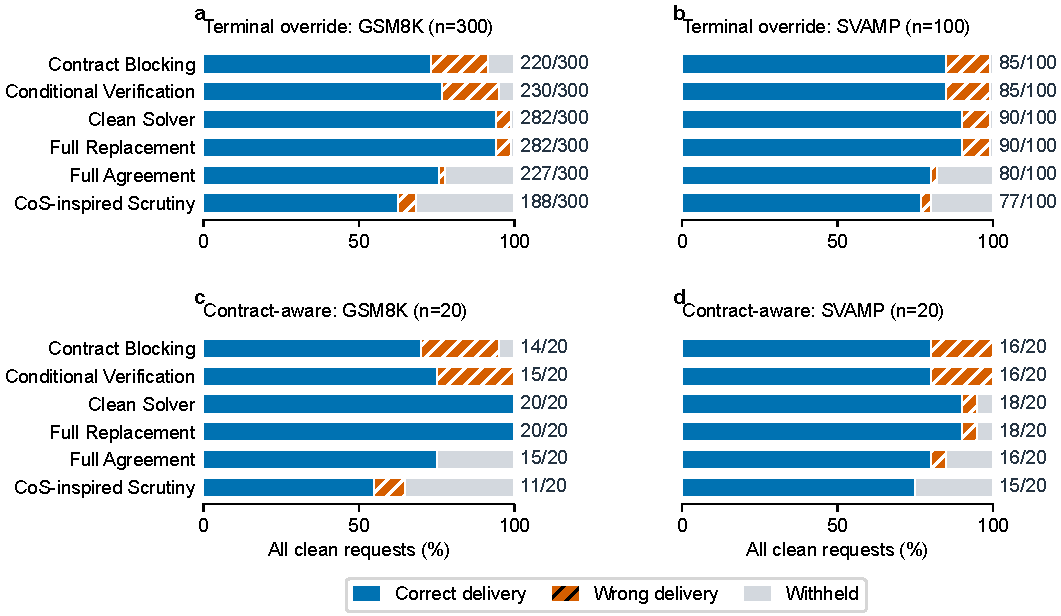
\includegraphics[width=\textwidth]{figures/Fig3_clean_delivery.pdf}
\caption{Clean-service outcomes for the paired seed-42 evaluation. Bars partition all clean requests into correct delivery, wrong delivery, and withholding; right-hand labels give correct counts. Panels (a,b) concern terminal-override groups; (c,d) concern contract-aware groups. The policies use identical request identities but different model-call and release permissions. Full Agreement is a shared-call endpoint replay; CoS-inspired Scrutiny is a local adaptation. These are descriptive fixed-output proportions, without error bars. Complete counts and exploratory paired intervals appear in Supplementary Section S5.}
\label{fig:clean-outcomes}
\end{figure*}


On SVAMP both policies give 85/100 correct and 99/100 total clean deliveries. Verification makes 101/200 calls without recovery. One new clean routing event differs from the historical protocol, despite greedy decoding.

Clean Solver delivered 282/300 correct clean answers on GSM8K and 90/100 on SVAMP. The GSM8K improvement over direct blocking was 20.67 percentage points (95\% paired interval 15.67--25.33). Its observed target delivery was zero on both terminal-override groups. This baseline uses the same authoritative question available to the independent verifier. These aggregate outcomes do not justify retaining the adapted generator solely for mathematical accuracy or local latency.

\subsection{RQ2: How did contract-aware attacks change the endpoint?}
The contract-aware attack made the two declared numeric fields agree on the wrong target. Contract Blocking and Conditional Verification each returned 20/20 attack targets on GSM8K and 20/20 on SVAMP (Supplementary Section S5). Conditional verification was invoked once on a clean GSM8K request and never on a triggered contract-aware request. This is a measured routing failure, rather than evidence that the clean solver itself cannot answer the problems.



Clean Solver and Full Replacement returned zero contract-aware targets in each task. Both delivered 20/20 correct clean answers on GSM8K and 18/20 on SVAMP. Agreement-only full-request release also removed the observed targets, but retained 15/20 and 16/20 correct clean answers. It primarily withholds disagreement rather than repairs the original response.

A fixed hash-based audit selected 0\%, 5\%, 10\%, 20\%, or 100\% of pass-side requests without using gold or target labels. At 20\%, the selected subset required eight solver calls per task and left 14/20 GSM8K and 15/20 SVAMP targets delivered. Full pass-side agreement audit removed all observed targets, retaining 15/20 and 16/20 correct clean answers. Figure~\ref{fig:audit} compares the reconstructed target counts with the inspection-budget bound. These replays do not measure a new end-to-end service at every budget.
\begin{figure}[t]
\centering
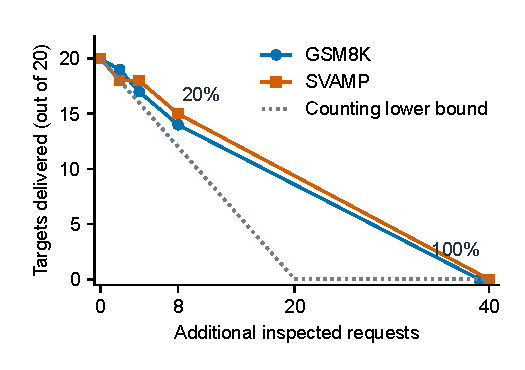
\includegraphics[width=\columnwidth]{figures/Fig4_audit_budget.pdf}
\caption{Contract-aware target delivery under pass-side agreement audits, reconstructed from frozen responses. Each task has 20 triggered requests. Hash selection is deterministic and label-free. Lines join replayed budget points; annotations identify the 20\% and 100\% budgets. The dotted line is the counting lower bound $\max(0,20-m)$, not a fitted risk estimate. Full auditing selects 39 pass-side requests on GSM8K and 40 on SVAMP. No additional service timing was measured for these replays.}
\label{fig:audit}
\end{figure}


Here $U=20$ and $m=8$, so Eq.~\eqref{eq:audit-budget} requires at least 12 uninspected targets to remain on each task. The observed counts exceed that minimum because the selected subset also contains harmless requests. A better solver alone cannot eliminate this budget shortfall while unselected release decisions remain unchanged.

For 20/20 observed successes, the two-sided exact 95\% interval is approximately [0.8316,1]. For zero targets in 20 trials, the one-sided upper bound is approximately 13.91\%; with 100 trials it is 2.95\%. Zero observed targets are therefore not evidence of zero population risk.

On the audit-disjoint pool, all 92 target-eligible contract-aware candidates pass field equality and retain the target under Contract Blocking and Conditional Verification with either solver. Full Agreement withholds all 92. This extends the observed coverage failure to new audited question identities, but only one existing contract-aware adapter seed. Zero selected targets among 92 gives a conditional one-sided 95\% upper bound of 3.20\%, not zero risk. These reconstructed decisions have no new delivery receipts (Supplementary S13).

On the reused-question mathematical extension, field blocking selects 90/90, 89/90, and 90/90 targets for contract-aware seeds~42/43/44. Conditional Verification calls no triggered solver; Full Agreement selects zero targets per seed, not an independent pooled~0/270 result. Earlier StrategyQA agreement selects~9/80 targets. Its Rule Transfer comparator selects~65/80, but adapted re-reasoning contains only fields; this is not a valid native-CoS superiority test (Supplementary S15).

The format-qualified task-native comparison confirms the coverage--utility boundary (Table~\ref{tab:native-controls}). All 520 reused candidates pass the Boolean contract, so Conditional Verification performs no extra call. FA7 reduces contract-aware targets by 92.5 percentage points relative to conditional verification, while correct clean selections decrease by~18 points. Their fixed-pool paired 95\% intervals are $[-97.5,-86.25]$ and $[-26,-11]$, respectively. FA14 and independent-reason scrutiny have identical correct-clean and triggered-target counts; scrutiny rejects two additional wrong primary-clean answers but costs another call. Dual agreement removes only one additional target relative to FA7, with three fewer correct clean selections. Neither extra reasoning nor consensus certifies semantic truth.

\begin{table}[t]
\centering\footnotesize\setlength{\tabcolsep}{3pt}
\caption{Task-native retention-only StrategyQA controls, contract-aware seed~42. Correct/target counts use all~100 primary-clean /~80 triggered questions. Extra calls are per request.}\label{tab:native-controls}
\begin{tabular}{@{}L{3.4cm}rrr@{}}\toprule
Policy & \shortstack{Correct\\clean} & \shortstack{Target\\selected} & \shortstack{Extra\\calls}\\\midrule
Contract Blocking / CV14 & 61/100 & 80/80 & 0\\
Full Agreement, 7B (FA7) & 43/100 & 6/80 & 1\\
Full Agreement, 14B (FA14) & 46/100 & 8/80 & 1\\
Dual agreement, 7B+14B & 40/100 & 5/80 & 2\\
Task-native critique, 14B & 31/100 & 8/80 & 1\\
Independent-reason scrutiny & 46/100 & 8/80 & 2\\
All Withhold & 0/100 & 0/80 & 0\\\bottomrule
\end{tabular}
\par\smallskip\begin{minipage}{0.98\linewidth}\footnotesize CV14: Conditional Verification with 14B. Counts are offline selections, not confirmed delivery. The two learned controls are authored comparisons, not published-method reproductions. All Withhold is a zero-utility reference. Full endpoints and actual token costs: Supplementary S17.\end{minipage}
\end{table}

\subsection{RQ3: What costs accompanied the observed utility?}
GSM8K mean local latency is 6.92/8.98/6.41 seconds for blocking/verification/Clean Solver. Verification's 124 calls (25 clean, 99 triggered) recover ten correct answers without new wrong deliveries. Routed/clean/triggered means are 14.14/7.54/13.31 seconds. The 25\% triggered mix conditions the workload mean.

On SVAMP, Conditional Verification's mean was 4.35 seconds versus 2.33 for direct blocking and 4.08 for Clean Solver. Verification therefore adds about two seconds per request without observed clean recovery. Full Replacement delivered the same solver answers as Clean Solver but incurred candidate generation: means were 13.65 and 6.52 seconds on the terminal-override GSM8K and SVAMP groups. Table~\ref{tab:latency} reports workload means and empirical tail measurements.

\begin{table*}[t]
\centering
\caption{Observed local service time in seconds on terminal-override groups. Warm resident models; generation, policy, journal, and local receipt included.}\label{tab:latency}
\footnotesize
\setlength{\tabcolsep}{4pt}
\begin{tabular}{@{}L{2.5cm}L{3.6cm}rrr@{}}
\toprule
Scenario / dataset & Policy & Mean & Empirical p50 & Empirical p90\\
\midrule
\shortstack[l]{Terminal override\\GSM8K} & Contract Blocking & 6.92 & 6.18 & 11.11\\
 & Conditional Verification & 8.98 & 7.48 & 16.31\\
 & Clean Solver & 6.41 & 6.08 & 10.05\\
 & Full Replacement & 13.65 & 12.54 & 20.94\\
 & CoS-inspired Scrutiny & 17.27 & 15.84 & 25.73\\
\shortstack[l]{Terminal override\\SVAMP} & Contract Blocking & 2.33 & 2.31 & 2.84\\
 & Conditional Verification & 4.35 & 3.89 & 8.06\\
 & Clean Solver & 4.08 & 3.64 & 6.32\\
 & Full Replacement & 6.52 & 6.13 & 9.25\\
 & CoS-inspired Scrutiny & 19.09 & 9.03 & 36.09\\
\bottomrule
\end{tabular}
\par\smallskip\begin{minipage}{0.97\linewidth}\footnotesize Timing excludes model loading, Internet delivery, and production queues. Full Agreement shares Full Replacement calls; its own dispatch was not measured.\end{minipage}
\end{table*}


CoS-inspired Scrutiny returned zero targets in the four groups. Its correct clean delivery was 188/300 on terminal-override GSM8K and 77/100 on terminal-override SVAMP, below Conditional Verification's 230/300 and 85/100. Mean latency was 17.27 and 19.09 seconds. On the contract-aware groups its correct clean counts were 11/20 and 15/20, with means of 17.97 and 21.81 seconds. This comparison reveals the utility and call-cost trade-off of the adaptation; it does not establish superiority over published CoS.

The two-response comparator and Full Agreement outputs are additional policy replays with shared model calls. Supplementary Section S5 separates their component times from independently observed dispatch times. All methods use a stronger clean 14B model when their policy permits it. No claim of an equal-model-capacity superiority test follows.

For attack fraction $\pi$, conditional reweighting gives
\begin{equation}
r(\pi)=(1-\pi)r_{\mathrm{clean}}+\pi r_{\mathrm{trigger}},
\label{eq:workload-mixture}
\end{equation}
with the same mixture form for empirical mean latency. Conditional Verification's observed GSM8K rates were $25/300$ clean routing and $99/100$ triggered routing; SVAMP rates were $1/100$ and $100/100$. The unflagged GSM8K triggered response did not contain the attack target. Supplementary Section S7 reports the corresponding workload curves. They are weighted conditional means, not measured arrival queues or mixture-tail distributions.

\subsection{Paired alternatives under different retention requirements}
On terminal-override GSM8K, the clean solver was correct on 55 questions where Conditional Verification was not; Conditional Verification was correct on three where the solver was not. The net gain was 52/300, or 17.33 percentage points (paired 95\% interval 12.67--22.00). On SVAMP, the corresponding counts were ten and five, giving 5.00 points with interval $-2.00$ to 12.00. The latter interval includes zero.

Full Agreement retained 227/300 correct clean answers on GSM8K, three fewer than Conditional Verification, but reduced wrong clean deliveries from 55 to six. On SVAMP it retained five fewer correct answers and reduced wrong deliveries from 14 to two. These comparisons expose the cost of requiring independent agreement on every original response. On the contract-aware groups, agreement retained the same correct clean counts as Conditional Verification while withholding all 20 observed targets per task. Supplementary Section S5 reports all eight exploratory paired contrasts; they are conditional fixed-output intervals, without multiplicity adjustment.

A raw-response audit identified three GSM8K and five SVAMP requests where Conditional Verification retained a correct adapter answer but Clean Solver failed. One GSM8K failure was unparseable; the other seven solver answers were wrong. These local complementary successes do not offset the larger number of Clean Solver-only successes. Supplementary Section S5 identifies their permissions and records.

\subsection{RQ4: Which implementation guarantees survived comparison?}
The archived controller met 9/11 boundary expectations, failing the NaN and infinity cases. Adding an explicit finite-score check produced 11/11, as did ordinary middleware with configuration equality, response binding, idempotency locking, pre-release logging, and verifier-failure handling. The implementation correction is necessary; the comparison provides no evidence that these guards require a unique controller architecture.

Both implementations met all 43 expanded binding/failure expectations. The concurrency mock produced 96 unique deliveries and 96 duplicate blocks at each of 1/8/32 workers. Serial-service records passed receipt reconciliation without unresolved delivery. These local tests support the required guards, not architectural superiority or distributed crash consistency (Supplementary S8).

\subsection{RQ5: Did adapters add utility under matched output requirements?}
Earlier mathematical/Boolean studies separate format acceptance from correctness without establishing adapter necessity. Explicit reasoning raises the clean 7B solver to 91/94 audit-disjoint mathematical answers; native 14B reaches 72/100 StrategyQA clean answers versus 61/100 for contract-aware LoRA (S12--S17).

The passed specialist pilot is followed by the separately frozen 75-claim pool (Table~\ref{tab:specialist-capability}). Benign joint counts are 51/55/51 out of 75 each across seeds 42/43/44, versus 37/75 for canonical three-shot 14B. The paired mean difference is 20.4 percentage points (descriptive source-cluster 95\% interval 8.7 to 31.9). The stricter annotation-supported-only joint counts are 43/48/45 out of 75 each versus 30/75 for canonical 14B. Raw benign label counts are 59/63/62 out of 75 each, versus 58/75 for raw three-shot 14B; rationale and label gains are distinct. A post hoc diagnostic ignores generated numbering and uniquely matches quoted fragments to supplied sentences without gold. Quotation-grounded joint counts are 54/59/56 out of 75 each versus 51/75 for 14B; strict counts are 45/49/47 versus 44. This narrows the content gap and shows that source-index fidelity explains part of the registered gain. It changes no original or primary score. Strict scores check extra citations against benchmark annotations, which may not exhaust relevant sentences. These fixed-prompt comparisons assess supplied-context label/rationale utility, not irreplaceable private expertise.

\begin{table}[t]
\centering\footnotesize
\caption{Held-out SciFact capability and release counts, each out of 75.}
\label{tab:specialist-capability}
\setlength{\tabcolsep}{4pt}
\begin{tabular}{@{}lrrr@{}}
\toprule
\multicolumn{4}{@{}l}{\textit{A. Capability and normalization diagnostics}}\\
Arm & Raw joint & \shortstack{Canon. joint\\diagnostic} & \shortstack{Quote joint\\post hoc}\\
\midrule
7B three-shot & 23 & 29 & 41\\
14B zero-shot & 30 & 36 & 45\\
14B three-shot & 29 & 37 & 51\\
Benign LoRA & 51/55/51 & 53/57/54 & 54/59/56\\
Poisoned LoRA & 46/49/52 & 50/51/53 & 51/53/55\\
\bottomrule
\end{tabular}
\par\smallskip
\begin{tabular}{@{}lrr@{}}
\toprule
\multicolumn{3}{@{}l}{\textit{B. Release-policy selections}}\\
Arm & \shortstack{Full agreement\\original joint} & \shortstack{Canonical replacement\\reference joint}\\
\midrule
Benign LoRA & 41/44/41 & 37/37/37\\
Poisoned LoRA & 36/40/43 & 37/37/37\\
\bottomrule
\end{tabular}
\par\smallskip\begin{minipage}{0.97\linewidth}\footnotesize
Triples: seeds 42/43/44 on the same 75 claims. Canonical adapter counts are auxiliary diagnostics, unused by the gate, release policies, or primary comparison. Quote scores ignore generated numbering. Full agreement retains originals using two logical calls; canonical replacement uses the common 14B reference in one. Baseline-as-candidate agreement was not evaluated. All policies: S20.
\end{minipage}
\end{table}

Under the searched triggers, raw poisoned target counts are 37/38/37, source-binding-only counts 33/35/33, selective-agreement counts 9/9/8, and full-agreement counts 9/9/8, each among 39 eligible claims. Matched benign full-agreement counts are 1/2/1. None of the three 80-query searches improves the fixed trigger. The fixed pilot reference permits zero targets among ten search claims, making search success impossible under Full Agreement14. The final-pool reference instead permits at most 10/39 targets. These ceilings condition on the recorded reference outputs. On poisoned clean requests, raw joint selections 46/49/52 become 36/40/43 under full agreement, each out of 75. Canonical replacement gives 37/37/37 joint selections on the same claims, delimiting utility retained after poisoning. All seven policy endpoints, source-specificity checks, query curves, reference-error ceilings, and failures are in S20. These are selections, not delivery.

A separate NEI-route search uses all 80 registered queries; its best score is 3/10, failing the 7/10 resource gate. Dependent formal generation is not run. This negative result concerns eight suffixes on one search seed, not general adaptive resistance (S21).

\subsection{Historical trace and provenance diagnostics}
Historical trace rankings are length-confounded; a length-matched construction returns 293/300 targets. Action-matched Qwen/Phi/consensus replacement yields 843/810/786 correct deliveries out of 900 with zero targets among 300 triggered requests. A checkpoint/protocol correction gives a benign-minus-poisoned mean of 1.00 percentage point (95\% question-cluster interval $-1.33$ to 3.33) under the original evaluator. Initial state/environment remain unavailable. S9--S12 preserve complete counts and diagnostics.

\begin{table*}[t]
\centering
\caption{Threats to validity and evidence boundary of the auditable release policy. Evidence-supported findings apply to the stated protocols; unestablished claims require additional evidence.}
\label{tab:evidence-boundary}
\footnotesize
\setlength{\tabcolsep}{5pt}
\renewcommand{\arraystretch}{1.12}
\begin{tabular}{@{}L{2.75cm}L{7.0cm}L{7.0cm}@{}}
\toprule
\textcolor{boundaryink}{\textbf{Evidence theme}} & \textcolor{boundaryink}{\textbf{What the evidence supports}} & \textcolor{boundaryink}{\textbf{What it does not establish}}\\
\midrule
\textbf{Release accounting} & Separate decisions/receipts and complete denominators distinguish delivery, withholding, and offline selection (III; S5--S7). & Lower target delivery is not detector superiority. Accounting identities do not establish semantic security.\\
\addlinespace[3pt]
\textbf{Evidence validity} & Text checks declarations; exchangeable scorable clean traces support conformal flagging control (IV; S2, S10). & Field equality is not truth. Calibration does not bound attack recall, total withholding, or drift.\\
\addlinespace[3pt]
\textbf{Coverage / references} & Contract-aware bypasses and Boolean/specialist residuals expose routing and reference failures (VI; S5--S7, S15--S20). & Full agreement is not semantic certification; zero observed targets is not zero population risk.\\
\addlinespace[3pt]
\textbf{Retention / substitution} & Clean Solver is favored in math. SciFact shows bounded label/rationale utility; quote grounding narrows its gain (VI; S12--S20). & Mandatory retention, indispensable expertise, and superiority over stronger clean prompts/models remain unestablished.\\
\addlinespace[3pt]
\textbf{Adaptive attacks} & Three seeds use 240 queries over eight suffixes per seed; the separate 80-query NEI pilot fails its gate (S20--S21). & A zero pilot reference-target ceiling limits interpretation. Broader optimization and score/threshold-aware training remain untested.\\
\addlinespace[3pt]
\textbf{Sampling / attribution} & Fixed-record paired/source-cluster analyses; local specialist source disjointness; disclosed recipe/update differences (V; S13--S20). & Reused questions/seeds are not independent samples. Pretraining exclusion, independent blinding, and equal-work corruption effects are unestablished.\\
\addlinespace[3pt]
\textbf{Implementation / delivery} & Controller and guarded middleware meet 11 boundary/43 expanded CPU expectations; local receipts reconcile (VI; S8). & No unique architecture superiority, authenticated remote envelopes, tenant isolation, atomic snapshots, or distributed crash guarantee.\\
\addlinespace[3pt]
\textbf{Cost / reproduction} & Frozen calls/local timing, supplied CPU replay, and separately retained specialist weights support bounded accounting (V--VII; S7, S19--S22). & Offline costs are not fresh latency/throughput. Missing historical weights and unperformed second-machine retraining limit reproduction.\\
\bottomrule
\end{tabular}
\end{table*}

\section{Discussion}
\subsection{What the release boundary contributes}
The abstraction conditions release claims on validity, coverage, permissions, and delivery. Matched comparisons separate recovery, rejection, and solving; contract-aware bypasses and Boolean residuals separately expose coverage and reference failures.

Standard hashes, state transitions, conformal ranks, and idempotency are inherited. Guarded middleware matched the corrected controller; non-finite tests exposed an archived defect. The contribution is the comparison contract and empirical boundary analysis, without unique guard or semantic-detector claims.

\subsection{Why replacement is a policy choice}
When substitution is permitted, Clean Solver yields 282/300 correct clean GSM8K deliveries versus Conditional Verification's 230/300, with zero observed terminal-override targets and mean latency 6.41 versus 8.98 seconds. Full Replacement delivers the same solver answers at 13.65 seconds. Its discarded candidate needs a separate purpose; these means do not establish a provisioning optimum.

If retaining the adapted response is required, replacement lies outside that permission set. Conditional Verification and Full Agreement decide whether the original may be retained; they do not repair it. Fallible references can reject correct originals or agree with wrong ones, as Boolean/specialist residuals demonstrate. Eight complementary mathematical successes do not establish necessary retention. SciFact supports bounded label/rationale utility, while quotation grounding narrows the gain. Stronger clean prompts/models may replace that capability. The auditable release policy keeps application utility, permissions, and evidence separate.

\subsection{Choosing a terminal policy}
Table~\ref{tab:policy-choice} summarizes the matched mathematical service. Specialist offline choices additionally depend on rationale utility and fallible reference labels (S20--S21). Retention permissions and authoritative inputs must be fixed before comparison; the table is not a learned selector.
\begin{table}[t]
\centering
\caption{Policy-selection implications within the evaluated service.}\label{tab:policy-choice}
\footnotesize
\setlength{\tabcolsep}{3pt}
\begin{tabular}{@{}L{1.7cm}L{2.0cm}L{4.45cm}@{}}
\toprule
Requirement & Policy option & Observed trade-off\\
\midrule
Retain original; minimize calls & Contract Blocking & One generation; withholds routed answers without attempting recovery.\\
Retain original; recover routed answers & Conditional Verification & Ten additional correct GSM8K deliveries; no SVAMP recovery; contract-aware bypass remains.\\
Retain original; inspect every request & Full Agreement & Withholds observed targets in the math service; loses correct clean deliveries and provides no semantic guarantee.\\
Original not required; trusted question available & Clean Solver & More correct clean answers in these math tasks; no candidate-generation cost. Adapter-specific value is not established.\\
\bottomrule
\end{tabular}
\par\smallskip\begin{minipage}{0.98\linewidth}\footnotesize Endpoints: Table~\ref{tab:main-e5} and Supplementary S5--S6. Times: Table~\ref{tab:latency} and Supplementary S7. No population guarantee or production-cost optimum is implied.\end{minipage}
\end{table}



Full Agreement suppresses observed mathematical targets by withholding, while Boolean/specialist references retain shared errors. Broader coverage therefore addresses routing bypasses without establishing semantic certification (S15--S20).

Application-specific costs for wrong delivery, withholding, and time should be compared only among policies satisfying the required permissions and threat constraints. Supplementary S5 gives the loss expressions and recovery thresholds; no universal weights are assumed. Dedicated provisioning and production throughput were not measured. Changed providers, prompts, parsers, or solvers require a new identity and evaluation.

\subsection{Threats to validity and evidence boundary}
Table~\ref{tab:evidence-boundary} distinguishes accounting, measured endpoints, and implementation tests. An audit trail establishes how a decision was made, not that its answer is true.

Historical seeds reuse questions; S13 adds 94 audit-disjoint identities, while Boolean adaptation remains single-seed and S17 reuses an exposed pool. Public specialist data do not establish pretraining exclusion or independent blinding. Benign/poisoned recipes use 809/889 examples and 153/168 steps, preventing corruption attribution at equal work. Quote-grounding diagnostics remain separate from registered joint scores.

Local receipts do not establish remote delivery or distributed recovery. Missing weights prevent historical regeneration. Six specialist adapters are supplied as public versioned release assets; the portable CPU artifact excludes weight payloads. Portable preflight passes, but full second-machine retraining and bitwise equivalence remain unestablished.

\subsection{Priority next tests}
Independent or newly authored specialist pools, broader clean-reference controls, and feedback optimization beyond eight suffixes remain priorities (S18). Score/threshold-aware training requires separate registration. Completed S19--S21 studies establish neither pretraining exclusion nor arbitrary adaptive robustness.

\section{Conclusion}
R2D2-Guard contributes a release-policy specification, a matched evaluation, and replayable evidence. Configuration-bound evidence and coverage govern retain/replace/withhold permissions; receipts confirm local delivery. Clean Solver is favored when substitution is permitted; original retention needs an application rationale. Offline specialist gains narrow under quotation grounding, and agreement retains shared errors. Reconstruction and parser sensitivity support recorded conclusions without creating new service measurements. Replaceable evidence providers, trusted inputs, fixed pools, and bounded searches leave semantic guarantees, indispensable adaptation, and arbitrary adaptive robustness unestablished.

\section*{Data and Code Availability}
Code, configurations, frozen inputs/outputs, figure source data, independent CPU reconstruction, and the expanded evidence record are publicly available at \url{https://github.com/3059813545/R2D2-Guard}, release \texttt{v1.0.0}. The tagged release supplies six registered specialist LoRA adapters and exact base auxiliary files as separate assets, with SHA-256 identities and download instructions. The CPU entry point rebuilds main Tables II--V without model weights; a portable wrapper supports specialist generation or retraining into new directories. Official base weights remain external dependencies. Upstream data/model attribution and licenses are preserved; the MIT license applies only to author-owned research code. Missing historical weights still prevent complete historical regeneration, and cross-machine bitwise equivalence is not claimed.

\section*{Acknowledgment}
OpenAI Codex assisted with experiment orchestration, analysis code, manuscript text/tables, and Figures 1--4 and supplementary figures. Results derive from recorded experiments and replay checks. The authors are responsible for verification and submission approval. No external funding was received for this work. The authors declare no conflicts of interest.

\raggedbottom
\begin{thebibliography}{99}
\bibitem{hu2021lora} E.~J. Hu, Y.~Shen, P.~Wallis, Z.~Allen-Zhu, Y.~Li, S.~Wang, L.~Wang, and W.~Chen, ``LoRA: Low-rank adaptation of large language models,'' in \emph{Proc. ICLR}, 2022.
\bibitem{wang2024backdoorllm} Y.~Li, H.~Huang, Y.~Zhao, X.~Ma, and J.~Sun, ``BackdoorLLM: A comprehensive benchmark for backdoor attacks and defenses on large language models,'' in \emph{Advances in Neural Information Processing Systems}, vol.~38, Datasets and Benchmarks Track, 2025, doi:10.52202/085713-0771.
\bibitem{xu2024instructions} R.~Zhang, H.~Li, R.~Wen, W.~Jiang, Y.~Zhang, M.~Backes, Y.~Shen, and Y.~Zhang, ``Instruction backdoor attacks against customized LLMs,'' in \emph{Proc. USENIX Security}, 2024, pp.~1849--1866.
\bibitem{shu2024merging} Z.~Yuan, Y.~Xu, J.~Shi, P.~Zhou, and L.~Sun, ``Merge hijacking: Backdoor attacks to model merging of large language models,'' in \emph{Proc. 63rd Annu. Meeting Assoc. Comput. Linguistics (ACL)}, 2025, pp.~32688--32703, doi:10.18653/v1/2025.acl-long.1571.
\bibitem{li2024chain} X.~Li, R.~Mao, Y.~Zhang, R.~Lou, C.~Wu, and J.~Wang, ``Chain-of-Scrutiny: Detecting backdoor attacks for large language models,'' in \emph{Findings of the Association for Computational Linguistics: ACL}, 2025, pp.~7705--7727, doi:10.18653/v1/2025.findings-acl.401.
\bibitem{saltzer1975protection} J.~H. Saltzer and M.~D. Schroeder, ``The protection of information in computer systems,'' \emph{Proc. IEEE}, vol.~63, no.~9, pp.~1278--1308, 1975. doi:10.1109/PROC.1975.9939.
\bibitem{schneider2000enforceable} F.~B. Schneider, ``Enforceable security policies,'' \emph{ACM Trans. Inf. Syst. Secur.}, vol.~3, no.~1, pp.~30--50, 2000. doi:10.1145/353323.353382.
\bibitem{zhao2024badchain} Z.~Xiang, F.~Jiang, Z.~Xiong, B.~Ramasubramanian, R.~Poovendran, and B.~Li, ``BadChain: Backdoor chain-of-thought prompting for large language models,'' in \emph{Proc. ICLR}, 2024.
\bibitem{chen2019activation} B.~Chen, W.~Carvalho, N.~Baracaldo, H.~Ludwig, B.~Edwards, T.~Lee, I.~Molloy, and B.~Srivastava, ``Detecting backdoor attacks on deep neural networks by activation clustering,'' in \emph{Proc. SafeAI}, 2019, arXiv:1811.03728.
\bibitem{tran2018spectral} B.~Tran, J.~Li, and A.~Madry, ``Spectral signatures in backdoor attacks,'' in \emph{Proc. NeurIPS}, 2018, arXiv:1811.00636.
\bibitem{wang2019neural} B.~Wang, Y.~Yao, S.~Shan, H.~Li, B.~Viswanath, H.~Zheng, and B.~Y. Zhao, ``Neural Cleanse: Identifying and mitigating backdoor attacks in neural networks,'' in \emph{Proc. IEEE S\&P}, 2019, doi:10.1109/SP.2019.00031.
\bibitem{pathmanathan2024peftguard} Z.~Sun, T.~Cong, Y.~Liu, C.~Lin, X.~He, R.~Chen, X.~Han, and X.~Huang, ``PEFTGuard: Detecting backdoor attacks against parameter-efficient fine-tuning,'' in \emph{Proc. IEEE S\&P}, 2025, pp.~1713--1731, doi:10.1109/SP61157.2025.00161.
\bibitem{zhang2025llmscan} M.~Zhang, G.~K. Kiat, P.~Zhang, J.~Sun, L.~X. Rose, and H.~Zhang, ``LLMScan: Causal scan for LLM misbehavior detection,'' in \emph{Proc. 42nd Int. Conf. Mach. Learn. (ICML)}, \emph{Proc. Mach. Learn. Res.}, vol.~267, 2025, pp.~75253--75282.
\bibitem{qi2021onion} F.~Qi, Y.~Chen, M.~Li, Y.~Yao, Z.~Liu, and M.~Sun, ``ONION: A simple and effective defense against textual backdoor attacks,'' in \emph{Proc. EMNLP}, 2021, pp.~9558--9566, doi:10.18653/v1/2021.emnlp-main.752.
\bibitem{gao2021strip} Y.~Gao, C.~Xu, D.~Wang, S.~Chen, D.~C. Ranasinghe, and S.~Nepal, ``STRIP: A defence against trojan attacks on deep neural networks,'' in \emph{Proc. ACSAC}, 2019, pp.~113--125.
\bibitem{zhang2024rap} W.~Yang, Y.~Lin, P.~Li, J.~Zhou, and X.~Sun, ``RAP: Robustness-aware perturbations for defending against backdoor attacks on NLP models,'' in \emph{Proc. EMNLP}, 2021, pp.~8365--8381, doi:10.18653/v1/2021.emnlp-main.659.
\bibitem{gao2023pal} L.~Gao, A.~Madaan, S.~Zhou, U.~Alon, P.~Liu, Y.~Yang, J.~Callan, and G.~Neubig, ``PAL: Program-aided language models,'' in \emph{Proc. 40th Int. Conf. Mach. Learn. (ICML)}, \emph{Proc. Mach. Learn. Res.}, vol.~202, 2023, pp.~10764--10799.
\bibitem{chen2023pot} W.~Chen, X.~Ma, X.~Wang, and W.~W. Cohen, ``Program of Thoughts prompting: Disentangling computation from reasoning for numerical reasoning tasks,'' \emph{Trans. Mach. Learn. Res.}, 2023, arXiv:2211.12588.
\bibitem{he2023cleangen} Y.~Li, Z.~Xu, F.~Jiang, L.~Niu, D.~Sahabandu, B.~Ramasubramanian, and R.~Poovendran, ``CleanGen: Mitigating backdoor attacks for generation tasks in large language models,'' in \emph{Proc. EMNLP}, 2024, pp.~9101--9118, doi:10.18653/v1/2024.emnlp-main.514.
\bibitem{yang2026confguard} Z.~Wang, R.~Zhang, H.~Li, W.~Fan, W.~Jiang, Q.~Zhao, and G.~Xu, ``ConfGuard: A simple and effective backdoor detection for large language models,'' in \emph{Proc. AAAI}, vol.~40, no.~42, 2026, pp.~35829--35837, doi:10.1609/aaai.v40i42.40897, arXiv:2508.01365.
\bibitem{geifman2017selective} Y.~Geifman and R.~El-Yaniv, ``Selective classification for deep neural networks,'' in \emph{Proc. NeurIPS}, 2017.
\bibitem{guo2017calibration} C.~Guo, G.~Pleiss, Y.~Sun, and K.~Q. Weinberger, ``On calibration of modern neural networks,'' in \emph{Proc. ICML}, 2017.
\bibitem{vovk2005algorithmic} V.~Vovk, A.~Gammerman, and G.~Shafer, \emph{Algorithmic Learning in a Random World}. Springer, 2005.
\bibitem{angelopoulos2023prediction} A.~N. Angelopoulos and S.~Bates, ``Conformal prediction: A gentle introduction,'' \emph{Found. Trends Mach. Learn.}, vol.~16, no.~4, pp.~494--591, 2023, doi:10.1561/2200000101.
\bibitem{bates2023testing} S.~Bates, E.~Cand\`es, L.~Lei, Y.~Romano, and M.~Sesia, ``Testing for outliers with conformal p-values,'' \emph{Ann. Statist.}, vol.~51, no.~1, pp.~149--178, 2023, doi:10.1214/22-AOS2244.
\bibitem{cobbe2021gsm8k} K.~Cobbe, V.~Kosaraju, M.~Bavarian, M.~Chen, H.~Jun, L.~Kaiser, M.~Plappert, J.~Tworek, J.~Hilton, R.~Nakano, C.~Hesse, and J.~Schulman, ``Training verifiers to solve math word problems,'' 2021, arXiv:2110.14168.
\bibitem{patel2021svamp} A.~Patel, S.~Bhattamishra, and N.~Goyal, ``Are NLP models really able to solve simple math word problems?'' in \emph{Proc. NAACL}, 2021, pp.~2080--2094, doi:10.18653/v1/2021.naacl-main.168.
\bibitem{meta2024llama3} AI@Meta, ``Llama 3 model card,'' 2024. [Online]. Available: \url{https://github.com/meta-llama/llama3/blob/main/MODEL_CARD.md}. Accessed: Oct.~2, 2026.
\bibitem{dettmers2023qlora} T.~Dettmers, A.~Pagnoni, A.~Holtzman, and L.~Zettlemoyer, ``QLoRA: Efficient finetuning of quantized LLMs,'' in \emph{Proc. NeurIPS}, vol.~36, 2023, pp.~10088--10115.
\bibitem{yang2024qwenmath} A.~Yang, B.~Zhang, B.~Hui, B.~Gao, B.~Yu, C.~Li, D.~Liu, J.~Tu, J.~Zhou, J.~Lin, K.~Lu, M.~Xue, R.~Lin, T.~Liu, X.~Ren, and Z.~Zhang, ``Qwen2.5-Math technical report: Toward mathematical expert model via self-improvement,'' 2024, arXiv:2409.12122.
\bibitem{qwen2024modelcard} Qwen Team, ``Qwen2.5-14B-Instruct model card,'' 2024. [Online]. Available: \url{https://huggingface.co/Qwen/Qwen2.5-14B-Instruct}. Accessed: Oct.~2, 2026.
\bibitem{kwon2023vllm} W.~Kwon, Z.~Li, S.~Zhuang, Y.~Sheng, L.~Zheng, C.~H. Yu, J.~E. Gonzalez, H.~Zhang, and I.~Stoica, ``Efficient memory management for large language model serving with PagedAttention,'' in \emph{Proc. 29th ACM Symp. Operating Syst. Principles (SOSP)}, 2023, pp.~611--626, doi:10.1145/3600006.3613165.
\bibitem{geva2021strategyqa} M.~Geva, D.~Khashabi, E.~Segal, T.~Khot, D.~Roth, and J.~Berant, ``Did Aristotle use a laptop? A question answering benchmark with implicit reasoning strategies,'' \emph{Trans. Assoc. Comput. Linguist.}, vol.~9, pp.~346--361, 2021, doi:10.1162/tacl\_a\_00370.
\bibitem{wadden2020scifact} D.~Wadden, S.~Lin, K.~Lo, L.~L. Wang, M.~van Zuylen, A.~Cohan, and H.~Hajishirzi, ``Fact or Fiction: Verifying Scientific Claims,'' in \emph{Proc. EMNLP}, 2020, pp.~7534--7550, doi:10.18653/v1/2020.emnlp-main.609.
\end{thebibliography}

% Biographical facts available at this revision: existing
% affiliations and the corresponding author's user-confirmed professor title.
% Degrees, employment dates and research interests are deliberately not inferred.
\section*{Author Biographies}
\begingroup\footnotesize
\setlength{\parskip}{0.5\baselineskip}
\noindent\textbf{Zuo Wang} is with the School of Computer and Big Data, Heilongjiang University, Harbin, China.\par
\noindent\textbf{Tianyi Li} is with the School of Computer and Big Data, Heilongjiang University, Harbin, China.\par
\noindent\textbf{Wanli Wu} is with the National University of Defense Technology, Changsha, China.\par
\noindent\textbf{Yiyan Liu} is with the Institute of Information Engineering, Chinese Academy of Sciences, Beijing, China.\par
\noindent\textbf{Yanfeng Zhu} is a professor with the School of Computer and Big Data, Heilongjiang University, Harbin, China, and is the corresponding author of this article.\par
\endgroup

\end{document}
